%!TEX root = ms.tex

In this section, we describe the module \py{rigid}, an implementation of
rigid monoidal categories.
We present \emph{snake removal}, the algorithm for normalising rigid diagrams, and its application to the semantics of \emph{pregroup grammars}.
Note that rigid categories are also called \emph{autonomous} \cite{JoyalStreet88,Delpeuch14a}, they are equivalent to the compact 2-categories of Preller, Lambek \cite{PrellerLambek07} with one object.

A (strict) monoidal category $\mathbf{C}$ is \emph{rigid} when every object $x$
has left and right adjoints $x^l$ and $x^r$ and four morphisms
$x \otimes x^l \xto{\epsilon} 1 \xto{\eta} x^l \otimes x$ and
$x^r \otimes x \xto{\epsilon'} 1 \xto{\eta'} x \otimes x^r$ depicted as cups and caps,
subject to $(\epsilon' \otimes 1_x) \circ (1_x \otimes \eta') = 1_x = (1_x \otimes \epsilon) \circ (\eta \otimes 1_x)$.
Note that any monoidal functor between rigid categories is isomorphic to a rigid functor, i.e. which sends cups to cups and caps to caps.

In a rigid category, left and right adjoints are unique up to a unique isomorphism.
They cancel each other --- i.e. $(x^l)^r = x = (x^r)^l$ --- and they are anti-homomorphisms of the tensor product --- i.e. $1^l = 1^r = 1$, $(x \otimes y)^l = y^l \otimes x^l$ and $(x \otimes y)^r = y^r \otimes x^r$.
Thus, the adjoint of a product can always be written as a product of adjoints.
Given a set of atomic types $\Sigma_0$, the objects of the free rigid category are given by lists of pairs $(x, n) \in \Sigma_0 \times \bb{Z}$ with the inclusion $\Sigma_0 \injects \Sigma_0 \times \bb{Z}$ defined by $x \mapsto (x, 0)$ and the adjoints $(x, n)^l = (x, n - 1)$ and $(x, n)^r = (x, n + 1)$.
We define a \emph{rigid signature} $\Sigma$ as a pair of sets $\Sigma_0, \Sigma_1$ with a pair of functions $\mathtt{dom}, \mathtt{cod} : \Sigma_1 \to (\Sigma_0 \times \bb{Z})^\star$,
then the free rigid category is given by the quotient $\mathbf{RC}(\Sigma) = \mathbf{MC}(\Sigma') / \cal{R}$
where $\Sigma'$ is the monoidal signature with $\Sigma'_0 = \Sigma_0 \times \bb{Z}$ and $\Sigma'_1 = \Sigma_1 + \set{\mathtt{cup}_x : x \otimes x^r \to 1, \mathtt{cap}_x : 1 \to x \otimes x^l}_{x \in \Sigma'_0}$.
The cups and caps for the unit are the identity, those for $x \otimes y$ are given by nesting the cups and caps of $x$ and $y$.
The relations $\cal{R}$ are given by the snake equation for every $x \in \Sigma'_0$:
\begin{center}
\begin{tikzpicture}[baseline=(O.base)]
\node (O) at (0, 1.0) {};
\node () at (0.25, 2.0) {$x$};
\node () at (1.25, 1.0) {$x^r$};
\node () at (2.25, 1.0) {$x$};
\draw [out=-90, in=90] (0, 2.0) to (0, 0.75);
\draw [out=180, in=90] (1.5, 1.5) to (1.0, 1.25);
\draw [out=0, in=90] (1.5, 1.5) to (2.0, 1.25);
\draw [out=-90, in=90] (1.0, 1.25) to (1.0, 0.75);
\draw [out=-90, in=90] (2.0, 1.25) to (2.0, 0.0);
\draw [out=-90, in=180] (0, 0.75) to (0.5, 0.5);
\draw [out=-90, in=0] (1.0, 0.75) to (0.5, 0.5);
\node () at (3.0, 1.0) {$\sim$};
\node () at (4.25, 2.0) {$x$};
\draw [out=-90, in=90] (4.0, 2.0) to (4.0, 0.0);
\node () at (5.0, 1.0) {$\sim$};
\node () at (8.25, 2.0) {$x$};
\node () at (6.25, 1.0) {$x$};
\node () at (7.25, 1.0) {$x^l$};
\draw [out=-90, in=90] (8.0, 2.0) to (8.0, 0.75);
\draw [out=180, in=90] (6.5, 1.5) to (6.0, 1.25);
\draw [out=0, in=90] (6.5, 1.5) to (7.0, 1.25);
\draw [out=-90, in=90] (6.0, 1.25) to (6.0, 0.0);
\draw [out=-90, in=90] (7.0, 1.25) to (7.0, 0.75);
\draw [out=-90, in=180] (7.0, 0.75) to (7.5, 0.5);
\draw [out=-90, in=0] (8.0, 0.75) to (7.5, 0.5);
\end{tikzpicture}

\end{center}

The \py{rigid} module implements classes \py{Ty}, \py{Diagram}, \py{Box} and \py{Functor} which subclass those from \py{monoidal}.
Pregroup types, i.e. the objects of free rigid categories, are implemented as \py{Ty}-instances \py{x} with two attributes \py{x.l} and \py{x.r} for the adjoints.
\py{Box} has two subclasses \py{Cup} and \py{Cap} implementing the adjunction for simple types.
The \py{Diagram} class has two static methods \py{cups} and \py{caps} which implement the adjunction for product types.
The \py{normalize} and \py{normal\_form} methods are overriden to implement snake removal: for each pair of cup and cap forming a snake, we first apply interchangers to make them adjacent, then replace the snake with an identity, see \cite[Definition 2.12]{DunnVicary19}.

\begin{example}
A rigid category is compact-closed if it is also symmetric monoidal.
In that case, the left and right adjoints coincide.
The category of matrices over a commutative semiring with Kronecker product as tensor is compact-closed, thus it is rigid.
\end{example}

\begin{example}\label{example-pregroup}
Lambek's pregroup grammars \cite{Lambek99,Lambek01,Lambek08} can be defined in terms of free rigid categories.
Indeed, a pregroup is a thin rigid category, i.e. with at most one arrow between any two objects.
A pregroup grammar $G$ is given by a vocabulary $V$, a finite set of basic types $B$ with $s \in B$ the sentence type and a finite dictionnary $D \sub V \times (B \times \bb{Z})^\star$ assigning pregroup types to words.
Let $\Sigma_G$ be the rigid signature with generating objects $V + B$ and arrows $w \to t$ for each dictionnary entry $(w, t) \in D$ and $\mathbf{G} = \mathbf{RC}(\Sigma_G)$.
The language of $G$ is given by $L(G) = \set{u \in V^\star \ \vert \ \exists \ f : u \to s \in \mathbf{G}}$.
That is, a list of words $u \in V^\star$ is a grammatical sentence whenever there is a diagram $f = g \circ d$ with $d : u \to t$ a product of dictionnary entries and $g : t \to s$ a pregroup derivation generated by cups and caps.
We do not draw the wires for words and depict the dictionnary entries as triangles. For example, let $B = \set{s, n}$ and $D = \set{\text{one, two, three} \to n, \s \text{plus} \to n^r \otimes n \otimes n^l, \s \text{equals} \to n^r \otimes s \otimes n^l}$, then ``one plus two equals three'' is a grammatical sentence:
\begin{center}
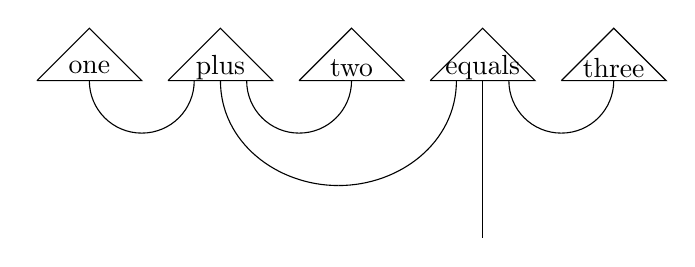
\begin{tikzpicture}[baseline=(O.base), scale=0.666]
\node (O) at (0, 0) {};
\draw (0.0, 0) -- (2.0, 0) -- (1.0, 1) -- (0.0, 0);
\node () at (1.0, 0.25) {one};
\draw (2.5, 0) -- (4.5, 0) -- (3.5, 1) -- (2.5, 0);
\node () at (3.5, 0.25) {plus};
\draw (5.0, 0) -- (7.0, 0) -- (6.0, 1) -- (5.0, 0);
\node () at (6.0, 0.25) {two};
\draw (7.5, 0) -- (9.5, 0) -- (8.5, 1) -- (7.5, 0);
\node () at (8.5, 0.25) {equals};
\draw (10.0, 0) -- (12.0, 0) -- (11.0, 1) -- (10.0, 0);
\node () at (11.0, 0.25) {three};
\draw [out=-90, in=180] (1.0, 0) to (2.0, -1);
\draw [out=-90, in=0] (3.0, 0) to (2.0, -1);
\draw [out=-90, in=180] (4.0, 0) to (5.0, -1);
\draw [out=-90, in=0] (6.0, 0) to (5.0, -1);
\draw [out=-90, in=180] (9.0, 0) to (10.0, -1);
\draw [out=-90, in=0] (11.0, 0) to (10.0, -1);
\draw [out=-90, in=180] (3.5, 0) to (5.75, -2);
\draw [out=-90, in=0] (8.0, 0) to (5.75, -2);
\draw [out=-90, in=90] (8.5, 0) to (8.5, -3);
\end{tikzpicture}

\end{center}
\end{example}

\begin{example}
For any monoidal category $\mathbf{C}$, there is a free rigid category $A(\mathbf{C})$ with a fully-faithful monoidal functor $\mathbf{C} \injects A(\mathbf{C})$, see \cite{Delpeuch14a}.
Concretely, this means that in a rigid diagram with boxes coming from a monoidal category, if the domain and codomain have no adjoint types then all snakes can be removed.
This allows to give a semantics to a pregroup grammar $G$ as a rigid functor $F : \mathbf{G} \to A(\mathbf{C})$.
For example, let $\text{one, two} : 1 \to n$ and $\text{plus} : n \times n \to n$ be functions, then we can compute the meaning of ``one plus two'':
\begin{center}
\begin{tikzpicture}[baseline=(O.base), scale=0.666]
\node (O) at (0, 3.5) {};
\node [scale=0.8] () at (0.5, 6.05) {$n$};
\node [scale=0.8] () at (2.5, 5.05) {$n^r$};
\node [scale=0.8] () at (4.5, 5.05) {$n$};
\node [scale=0.8] () at (6.5, 4.05) {$n$};
\node [scale=0.8] () at (8.5, 4.05) {$n^l$};
\node [scale=0.8] () at (5.5, 3.05) {$n$};
\node [scale=0.8] () at (10.5, 2.05) {$n$};
\draw (0.0, 6.25) .. controls (0.0, 1.75) .. (0.0, 1.75);
\draw (3.0, 5.5) .. controls (2.0, 5.5) .. (2.0, 5.25);
\draw (3.0, 5.5) .. controls (4.0, 5.5) .. (4.0, 5.25);
\draw (2.0, 5.25) .. controls (2.0, 1.75) .. (2.0, 1.75);
\draw (4.0, 5.25) .. controls (4.0, 3.75) .. (4.0, 3.75);
\draw (7.0, 4.5) .. controls (6.0, 4.5) .. (6.0, 4.25);
\draw (7.0, 4.5) .. controls (8.0, 4.5) .. (8.0, 4.25);
\draw (6.0, 4.25) .. controls (6.0, 3.75) .. (6.0, 3.75);
\draw (8.0, 4.25) .. controls (8.0, 0.75) .. (8.0, 0.75);
\draw (5.0, 3.25) .. controls (5.0, 0.0) .. (5.0, 0.0);
\draw (10.0, 2.25) .. controls (10.0, 0.75) .. (10.0, 0.75);
\draw (0.0, 1.75) .. controls (0.0, 1.5) .. (1.0, 1.5);
\draw (2.0, 1.75) .. controls (2.0, 1.5) .. (1.0, 1.5);
\draw (8.0, 0.75) .. controls (8.0, 0.5) .. (9.0, 0.5);
\draw (10.0, 0.75) .. controls (10.0, 0.5) .. (9.0, 0.5);
\draw (-0.5, 6.25) -- (0.5, 6.25) -- (0.5, 6.75) -- (-0.5, 6.75) -- (-0.5, 6.25);
\node [scale=0.8] () at (0, 6.5) {one};
\draw (3.5, 3.25) -- (6.5, 3.25) -- (6.5, 3.75) -- (3.5, 3.75) -- (3.5, 3.25);
\node [scale=0.8] () at (5.0, 3.5) {plus};
\draw (9.5, 2.25) -- (10.5, 2.25) -- (10.5, 2.75) -- (9.5, 2.75) -- (9.5, 2.25);
\node [scale=0.8] () at (10.0, 2.5) {two};
\node () at (12.0, 3.5) {$\mapsto$};
\node [scale=0.8] () at (14.5, 5.383333333333333) {$n$};
\node [scale=0.8] () at (16.5, 3.0500000000000003) {$n$};
\node [scale=0.8] () at (15.5, 0.7166666666666668) {$n$};
\draw (14.0, 5.583333333333333) .. controls (14.0, 1.4166666666666665) .. (14.0, 1.4166666666666665);
\draw (16.0, 3.2500000000000004) .. controls (16.0, 1.4166666666666665) .. (16.0, 1.4166666666666665);
\draw (15.0, 0.9166666666666667) .. controls (15.0, 0.0) .. (15.0, 0.0);
\draw (13.5, 5.583333333333334) -- (14.5, 5.583333333333334) -- (14.5, 6.083333333333334) -- (13.5, 6.083333333333334) -- (13.5, 5.583333333333334);
\node [scale=0.8] () at (14.0, 5.833333333333334) {one};
\draw (15.5, 3.25) -- (16.5, 3.25) -- (16.5, 3.75) -- (15.5, 3.75) -- (15.5, 3.25);
\node [scale=0.8] () at (16.0, 3.5) {two};
\draw (13.5, 0.9166666666666667) -- (16.5, 0.9166666666666667) -- (16.5, 1.4166666666666667) -- (13.5, 1.4166666666666667) -- (13.5, 0.9166666666666667);
\node [scale=0.8] () at (15.0, 1.1666666666666667) {plus};
\end{tikzpicture}
 $\quad \mapsto \quad 3$
\end{center}
where the first step is snake removal and the second is function evaluation as in appendix~\ref{3-cartesian}.
\end{example}
